% docs/learning_report/report.tex -- class project write-up (2026-11-15).
% Build: latexmk -pdf report.tex   (figures/tables from make_figures.py)
\documentclass[10pt]{article}
\usepackage[margin=0.7in]{geometry}
\usepackage{amsmath,amssymb}
\usepackage{graphicx}
\usepackage{booktabs}
\usepackage{float}
\usepackage[table]{xcolor}
\usepackage[numbers,sort&compress]{natbib}
\usepackage[font=small,labelfont=bf,skip=3pt]{caption}
\usepackage[colorlinks=true,linkcolor=blue!50!black,citecolor=blue!50!black,urlcolor=blue!50!black]{hyperref}
\usepackage{enumitem}
\usepackage{fancyvrb}
\setlist{nosep,leftmargin=1.3em}
\setlength{\textfloatsep}{8pt plus 2pt minus 2pt}
\setlength{\intextsep}{8pt plus 2pt minus 2pt}
\newcommand{\todo}[1]{\textcolor{red!70!black}{[#1]}}
\newcommand{\best}[1]{\cellcolor{green!22}#1}
\newcommand{\worst}[1]{\cellcolor{red!20}#1}
\newcommand{\dx}{\Delta x}

\title{Learning where coarse DSMC fails}
\author{Aakash Jain}
\date{November 2026}

\begin{document}
\maketitle

\begin{abstract}
Direct simulation Monte Carlo (DSMC) simulates rarefied gases with particles that collide inside
grid cells, and is accurate only when the cells are smaller than a mean free path. Cells
$8\times$ larger per direction need $64\times$ fewer particles in 2-D but make the simulated gas
too viscous and conductive. We train a per-cell correction to a cheap collision model, by
differentiating through the simulation, so that coarse cells reproduce fine-cell results, and
compare an interpretable lasso with a small neural network, both cross-validated over flows.
Inside the training conditions they are equally accurate; on the strongest unseen shock waves
the linear models are 1.5--2.7$\times$ worse than no correction while the network still improves
on it. Principal component analysis shows the nine physical inputs are strongly correlated, so lasso
coefficients cannot be reliably attributed to single mechanisms, and a nearest-neighbour
coverage score flags exactly the flows where the linear models fail. Against classical collision
schemes the learned model is best on shear flows but not on most shocks, where simulating binary
collisions directly is better. We recommend choosing the scheme per flow regime, with the network
behind the coverage check.
\end{abstract}

% =========================================================================================
\section{Introduction}

A gas is \emph{rarefied} when the mean free path $\lambda$, the average distance a molecule
travels between collisions, is not small compared with the flow features: around a satellite in
low orbit, a capsule entering the upper atmosphere, or in a micro-channel~\citep{boyd2017,
karniadakis2005}. The Navier--Stokes equations, which assume near-equilibrium, then fail, and the
gas obeys the Boltzmann equation for the distribution of molecular velocities~\citep{cercignani1988}.
It is solved by direct simulation Monte Carlo (DSMC)~\citep{bird1994,plimpton2019}: computational
particles, each standing for many molecules, move in straight lines for a time step; then
randomly chosen pairs within each grid cell collide with the probabilities of real molecular
collisions (Appendix~\ref{app:dsmc}).

DSMC is accurate only if each cell is smaller than about one mean free path. Collision partners
are picked anywhere in the same cell, so in a large cell two particles far apart can exchange
momentum and energy as if they had met. This spreads momentum and heat too easily: the simulated
viscosity grows as $\mu_\mathrm{eff}/\mu-1=\tfrac{16}{45\pi}(\dx/\lambda)^2$
\citep{alexander1998,hadjiconstantinou2000}, and the conductivity similarly. At a fixed number of particles per cell the cost is proportional to the number of cells, so
cells $8\times$ larger per direction save $64\times$ in 2-D and $512\times$ in 3-D (an idealised
count: real speed-ups also depend on the time step and the collision operator's own cost). Relaxation models
(BGK~\citep{bgk1954}, ES-BGK~\citep{holway1966}) and Fokker--Planck models~\citep{jenny2010,
gorji2011,mathiaud2016,fei2020} are cheaper: instead of simulating collisions they move each particle's velocity toward a
Gaussian (equilibrium) distribution at a rate set by the viscosity and conductivity, an
approximation that is best near equilibrium.

Neural networks have been trained to imitate the exact local collision process, as BGK
corrections~\citep{xiao2021,miller2022} or as a scattering law inside DSMC~\citep{roohi2026}. A
coarse cell has no exact local answer: what it should do is defined only by its effect on the
flow. We therefore train the correction \emph{through} the simulation, as is done for coarse-grid
turbulence models~\citep{um2020,kochkov2021,macart2021}; for DSMC this became possible only with
adjoint DSMC methods~\citep{caflisch2026}.

We correct the ES Fokker--Planck operator with velocity reconstruction (ES-FP+recon, the
``base''), which removes about half of the coarse-cell viscosity error on its own. A model reads
dimensionless properties of each cell and adjusts how its particles relax, with gradients from
automatic differentiation (AD) through a differentiable 2-D DSMC solver in JAX~\citep{jax2018}.
We compare an interpretable sparse linear model with a small neural network.

The decision this work supports is made by an engineer who must predict the drag and the
wall heating of a vehicle or device, and who chooses, for each flow, between (a)~a fine DSMC run,
(b)~a coarse run with a classical collision scheme, and (c)~a coarse run with a learned
correction (linear or neural). Trusting a coarse run where it is wrong (a false accept) can under-predict re-entry heating or
drag, at the cost of a vehicle or crew; running the fine simulation where a coarse one would do
(a false reject) costs 64--512 times more computation. A useful model needs a low error and a
cheap, reliable indication of \emph{where} it can be trusted.

We declared the baselines before any training, by running eight classical collision schemes on
every flow at the coarse cells. Every error below is a ratio to the base operator's error, so 1
means ``no better than learning nothing'', and the strongest classical schemes are reported
beside it. They are demanding baselines. NTC is the standard algorithm of production DSMC
codes~\citep{bird1994,plimpton2019}; NTC with nearest-neighbour (``adjacent'') pairing, which
picks collision partners close to each other, is the established remedy for the cell-size
error~\citep{bird1994}; ES-BGK and ES-FP with gradient reconstruction are relaxation methods with
the correct ratio of viscosity to conductivity (Prandtl number)~\citep{holway1966,mathiaud2016}.
No single one of the eight is best on every flow: BGK with reconstruction is best on the slow
shear wave, NTC on resolved shocks and adjacent pairing on strong shocks in coarse cells. A
learned model is worth using only where it beats all of them, which is a hard target.

% =========================================================================================
\section{Problem set-up}

The base operator moves each particle's velocity toward a Gaussian matching its cell's
temperature and stress; the stress decays at a rate $r_s$ and the heat flux at $r_q$, which set
the viscosity and conductivity, and the cell's mass, momentum and energy are restored exactly
(Appendix~\ref{app:dsmc}). For both the
linear model and the network, the output is $\delta=B\tanh(f(\phi)/B)$, with twelve components (two in the rate-only models): two multiply the rates by
$e^{\delta_s}$ and $e^{\delta_q}$ (effective viscosity and conductivity), seven set target
stress and heat flux from the local gradients (the second-order ``Burnett'' terms of kinetic
theory~\citep{chapman1970}), and three change the velocity interpolation within the cell and
the shape of the random part of the step. The $\tanh$ bound stops any input from driving a rate
to zero or infinity. We require $f_\theta(0)=0$ so that a well-resolved cell in equilibrium,
where the base is already right, is left unchanged.

\begin{table}[H]
\centering\footnotesize
\caption{Inputs, one per known error mechanism ($\lambda,\tau$: the cell's mean free path and
collision time~\citep{koura1991}; $N_c$ particles; $S$ strain rate), each divided by its RMS over
the training cells. Twelve-output models also read the signed $\lambda\nabla\!\cdot u/\sqrt\theta$
and $g\cdot Sg$ ($g=\lambda\nabla\ln T$), to tell compression from expansion.}
\label{tab:features}
\begin{tabular}{@{}llp{0.55\textwidth}@{}}
\toprule
name & definition & error mechanism it measures \\ \midrule
dx2, dx4 & $(\dx/\lambda)^2$, $(\dx/\lambda)^4$ & collision partners too far apart (cell
size)~\citep{alexander1998,hadjiconstantinou2000}, and its next order \\
dt2, dt1 & $(\Delta t/\tau)^2$, $\Delta t/\tau$ & time step too long compared with the collision
time~\citep{garcia2000} \\
inv\_n & $1/N_c$ & too few particles to estimate the cell's state~\citep{hadjiconstantinou2003} \\
dx2\_inv\_n & $(\dx/\lambda)^2/N_c$ & cell-size error estimated from a noisy cell \\
kn\_u2, kn\_t2 & $(\lambda|S|/v_\mathrm{th})^2$, $(\lambda|\nabla\ln T|)^2$ & velocity and
temperature change over one mean free path: departure from equilibrium~\citep{chapman1970} \\
dx2\_kn2 & $(\dx/\lambda)^2(\mathrm{Kn}_u^2+\mathrm{Kn}_T^2)$ & cell-size error growing with the
gradients \\
\bottomrule
\end{tabular}
\end{table}

Each input measures one known source of error, so that linear coefficients have a physical
meaning; all are dimensionless and local, so that one model can apply to any flow or density.

The training data come from twelve 2-D flows. The reference for each is a fine NTC simulation
with cells of $\lambda/4$. The coarse simulations use cells of $2\lambda$ for four decaying shear
waves (S1--S4: two amplitudes, $u_0/v_\mathrm{th}=0.1, 0.5$, times two wavelengths, $32\lambda$
and $128\lambda$), and cells of $\lambda_1$ or $4\lambda_1$, with $\lambda_1$ the upstream mean
free path, for eight normal shock waves (K1--K8: Mach 1.5, 3, 6 and 10, odd numbers at
$\lambda_1$, even at $4\lambda_1$). A shock is a jump in density, velocity and temperature a
few mean free paths thick; shocks stand for the flow ahead of an entering vehicle, shear waves
for the slow flows of micro-devices. We train on five flows, \textbf{S3, S4, K1, K4 and K8}, chosen to span both
families, both shock resolutions and the weakest and strongest shocks, and we keep the other
seven for testing. A final test that is never used for training or for choosing a model is a
Mach~10 cylinder simulated with the learned operator in every cell (Appendix~\ref{app:extra}).

Training runs short coarse simulations (100 steps) and measures the deviation $d$ of the coarse
stress and heat flux from the fine reference. The objective is the squared
\emph{average} deviation $\tfrac12\mathbb E[d]^2$, not the average of $d^2$, because $d^2$ also
contains the simulation's random noise, which a model could reduce by making the gas less random
rather than more correct. Its gradient $\mathbb E[d]\,\partial m/\partial\theta$ uses a running
estimate of $\mathbb E[d]$ and the exact derivative of the simulated fluxes $m$, from
reverse-mode AD through all 100 steps (Appendix~\ref{app:ad}).

Every result is an average over random particles, and a single training step's gradient is
about as large as its noise. We therefore evaluate models in separate simulations (512 independent runs per shear wave, 32
long independent runs per shock) and count a difference only beyond about two standard errors. A flow's
error is $|\mu/\mu_\mathrm{ref}-1|$ for a shear wave, where $\mu$ is the viscosity measured from
how fast the wave decays, and for a shock the root-mean-square of the errors in the total stress
and heat flux through the shock. We divide each error by the base operator's error on the same
flow and average these ratios geometrically, so that a halving and a doubling cancel. S1 is left
out of all averages because its base error ($0.06\pm0.05$) is smaller than its noise. This ratio measures fidelity, a proxy for the risk of a false accept rather than a measure of
it: deployment also needs an absolute, directional tolerance. For a heat shield sized with a 10\%
margin, a false accept is a coarse heat load more than 10\% \emph{below} the fine one, while an
over-prediction only costs mass (signed errors: Section~\ref{sec:decision}). Settings are chosen by \textbf{leave-one-case-out (LOCO)} cross-validation: train on four
training flows, measure the error on the fifth. We use flows as folds because the question is
whether a model works on a flow it has never seen; random folds would put the same flow into
both training and validation.

% =========================================================================================
\section{The interpretable model: a sparse linear correction}

The linear model is $\delta=B\tanh(A\phi/B)$, with the two rate adjustments as outputs and the nine inputs
of Table~\ref{tab:features}: eighteen coefficients, each the effect of one error mechanism on the
viscosity or the conductivity. To make it readable we added an $\ell_1$ (lasso)
penalty~\citep{tibshirani1996}, which sets unimportant coefficients exactly to zero. The
simulation makes the objective a nonlinear function of $A$, so we used a Gauss--Newton lasso:
around the current coefficients $A_0$ the deviation of each training window is approximated by a
straight line, $d(A)\approx d(A_0)+J(A-A_0)$, with the slope $J$ from forward-mode AD (2,048
windows per flow), and
\begin{equation}
\min_A\ \tfrac12\sum_\mathrm{flows}\overline{w\big(\bar d+\bar J(A-A_0)\big)^2}+\alpha\|A\|_1
\end{equation}
is solved by coordinate descent for 40 values of $\alpha$~\citep{friedman2010}. We chose
$\alpha$ with the one-standard-error rule~\citep{hastie2009} (the largest penalty whose
validation error is within one standard error of the best), because it prefers the simpler model
when the data cannot tell them apart. The validation error was computed by
LOCO and, as a weaker check, by splitting the reference data's random seeds in half; the fit was
re-linearised at the result three times.

\begin{figure}[H]
\centering
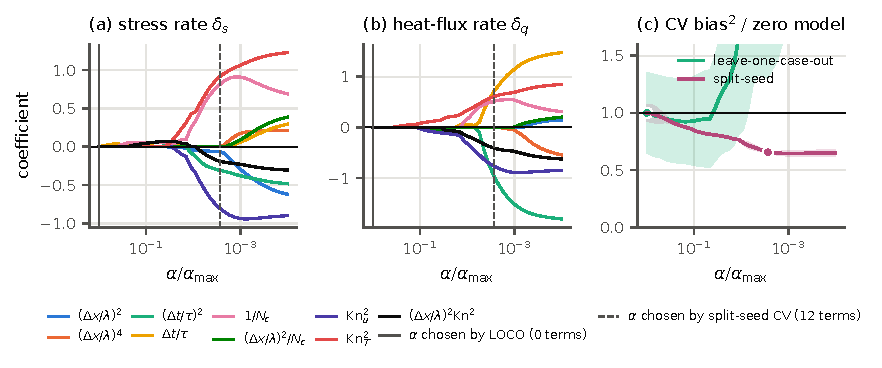
\includegraphics[width=\textwidth]{figures/fig_lasso.pdf}
\caption{Lasso coefficients as the penalty $\alpha$ is relaxed, for the stress rate (a) and
heat-flux rate (b); (c) validation error relative to no correction ($\pm1$ s.e.). LOCO (green;
solid line in a, b) selects no terms; the split-seed check (purple; dashed) selects 12 of the 18
(6 per panel) on this path, but 14 in a fresh solve at the same $\alpha$.}
\label{fig:lasso}
\end{figure}

The lasso did not produce a usable interpretable model (Figure~\ref{fig:lasso}). On unseen
flows its best was an 8\% improvement, within the noise, so the rule chose an empty model. On
unseen seeds of the same flows it kept 12--14 terms (the path and a fresh solve at the same
$\alpha$ disagree, a sign of ill-conditioning), and the Gauss--Newton steps became unstable: the
measured squared deviation after each step was 4--11 times the linear prediction, and
coefficients changed sign between steps. The lasso selected by cross-validation over flows is therefore the base operator itself. To
show what a non-empty lasso does, Table~\ref{tab:headline} keeps the final seven-term split-seed
fit as a diagnostic: it improves the training flows (0.76 of the base error) but is 2.7 times
worse than no correction on the strongest unseen shocks; Section~\ref{sec:why} shows why.

Although the fitted coefficients cannot be trusted, the order in which terms enter the path as
$\alpha$ is relaxed (Figure~\ref{fig:lasso}a, b) shows which inputs the path finds most useful first,
given those already in the model; it is not a ranking of standalone predictive power. The first five are, on the stress rate, the time step $\Delta t/\tau$ and particle count
$1/N_c$ (both positive: faster relaxation), on the heat-flux rate the temperature gradient
$\mathrm{Kn}_T^2$ (positive), then cell size times gradients on the stress rate (positive) and
$\mathrm{Kn}_u^2$ on the heat-flux rate (negative); the first three survive every bootstrap
resample.
The textbook cell-size term $(\dx/\lambda)^2$ enters only tenth, because the base's velocity
reconstruction already removes most of it. Two effects limit this reading: correlated inputs compete
for the same effect, so an early term may stand for a group (Section~\ref{sec:why}; three of the
first seven change sign along the path, and the first drops out and re-enters), and the path is fitted to noisy windows, with even the
first term not clearly supported across flows (LOCO).

We also trained unpenalised linear models like the network, on the two rates (0.67 of the base
error on the training flows) and on all twelve outputs (0.39). The latter is the like-for-like
comparison with the network. We did not run the lasso on the twelve outputs, because its
linearisation needs one forward-mode derivative per coefficient: 132 instead of 18.

% =========================================================================================
\section{The flexible model: a small neural network}

The network is $f_\theta(\phi)=\mathrm{MLP}(\phi)-\mathrm{MLP}(0)$, with $\tanh$ hidden layers
and a final layer initialised to zero, so training starts from the base operator. We tuned four
settings, each at three levels: the number of hidden layers (1, 2, 3), their width (8, 32,
128), the weight decay (0, $10^{-3}$, $10^{-2}$), which
shrinks the weights each step against overfitting~\citep{loshchilov2019}, and the Adam~\citep{kingma2015} learning rate ($10^{-3}$,
$3\times10^{-3}$, $10^{-2}$). We used an L9 orthogonal
array~\citep{hedayat1999} to save compute: nine settings instead of all 81, chosen so that every
pair of levels of any two settings appears exactly once. Each setting was trained seven times (five LOCO
folds, and twice on all five flows with different seeds): 63 runs on single GPU partitions.

\begin{figure}[H]
\centering
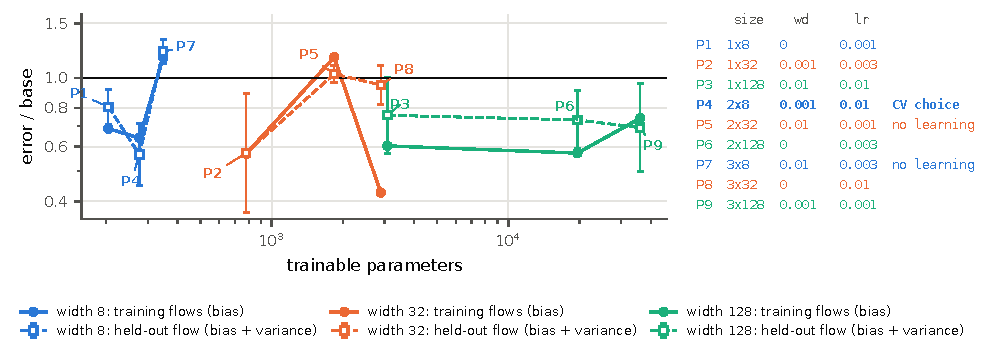
\includegraphics[width=0.78\textwidth]{figures/fig_mlp.pdf}
\caption{Error against network size: training flows (solid; bias) and the left-out flow, mean
over five LOCO folds $\pm1$ s.e. (dashed; bias plus variance). Lines join 1--3 hidden layers at
fixed width; P1--P9 label the settings listed on the right. Ratios use the full evaluation's
base error; the shorter validation runs read the
shock stress about 0.03 high, so the uncorrected operator itself scores 1.17 here.}
\label{fig:mlp}
\end{figure}

Figure~\ref{fig:mlp} shows the bias--variance trade-off only in part. With strong weight
decay and a small learning rate (two settings) the network never left the base. Among the settings that learned, more parameters lowered the training error: width 8
reached 0.64--0.69, width 32 and 128 mostly 0.57--0.60, and the three-layer, 32-wide network with
the largest learning rate and no weight decay reached 0.43. The error on unseen flows did not
follow. It stayed between 0.57 and 0.81 with no trend in size, and the three-layer 32-wide
network, the best on training flows, was among the worst on unseen ones (0.95): it overfits.
Held-out uncertainties (0.13--0.45 in log; five noisy folds) are as large as the differences
between settings. Two settings tie for the lowest held-out error (0.57): $1\times32$ ($\pm0.45$) and
$2\times8$ ($\pm0.23$). We chose \textbf{two layers of 8} (weight decay $10^{-3}$, learning rate
$10^{-2}$) for its smaller uncertainty and fewer parameters (276 against 780). We report it as
the geometric mean of the errors of its two all-flow training seeds, an estimate of what
retraining gives; a deployment uses one trained network, not an ensemble.

We also report a $2\times32$ network trained before this sweep. An earlier sweep with only the
two rate outputs had its best held-out error at $3\times32$, no weight decay, learning rate
$10^{-2}$, which also had the largest seed spread. As a first test of the twelve outputs we
trained two networks in that promising region, fixed before any unseen flow was evaluated: that
$3\times32$ setting, which was worse (0.50 on training flows, 0.70 on unseen shocks; it overfits
in Figure~\ref{fig:mlp}), and a $2\times32$ at an intermediate learning rate ($3\times10^{-3}$),
which, proposed from a different sweep, independently tests the cross-validated choice.

\begin{table}[H]
\centering\small
\caption{Error relative to the base (geometric mean over flows; green best, red worst per
column; ``out of range'': flagged by the coverage gate, Section~\ref{sec:why}). The 90\% intervals
cover particle noise for these flows and models, not variation across new flows or retraining.}
\label{tab:headline}
\resizebox{\textwidth}{!}{\begin{tabular}{@{}lcccc@{}}
\toprule
operator & training flows & held-out shear & held-out shocks, in range & held-out shocks, out of range \\
 & (5 flows) & S2 & K2, K3, K6 & K5, K7 \\
\midrule
NTC & 0.99 [0.77, 1.28] & \worst{1.90 [1.39, 2.59]} & \best{0.27 [0.13, 0.58]} & \best{0.05 [0.02, 0.11]} \\
NTC adjacent & 0.58 [0.42, 0.81] & 1.18 [0.83, 1.68] & 0.46 [0.36, 0.60] & 0.06 [0.03, 0.12] \\
BGK + recon & \worst{1.76 [1.38, 2.23]} & 0.56 [0.28, 1.12] & \worst{2.45 [2.07, 2.90]} & 1.89 [1.83, 1.95] \\
ES-BGK + recon & 0.60 [0.44, 0.84] & 1.11 [0.76, 1.62] & 0.53 [0.35, 0.79] & 0.61 [0.58, 0.65] \\
ES-FP + recon (base) & 1.00 [0.77, 1.30] & 1.00 [0.70, 1.42] & 1.00 [0.81, 1.24] & 1.00 [0.96, 1.04] \\
\midrule
linear, rate & 0.67 [0.52, 0.86] & 0.53 [0.31, 0.89] & 0.68 [0.52, 0.88] & 1.52 [1.47, 1.58] \\
lasso, rate (7-term diagnostic) & 0.76 [0.60, 0.97] & 0.55 [0.34, 0.88] & 0.47 [0.23, 0.99] & \worst{2.72 [2.64, 2.80]} \\
linear, rich & 0.39 [0.22, 0.71] & \best{0.21 [0.07, 0.60]} & 0.66 [0.48, 0.92] & 1.79 [1.72, 1.86] \\
MLP 2x8, rich (CV) & 0.43 [0.30, 0.62] & 0.35 [0.20, 0.59] & 0.50 [0.21, 1.19] & 0.71 [0.68, 0.73] \\
MLP 2x32, rich (pre-sweep) & \best{0.38 [0.14, 1.08]} & 0.34 [0.18, 0.67] & 0.45 [0.26, 0.79] & 0.69 [0.65, 0.72] \\
\bottomrule
\end{tabular}
}
\end{table}

Against their base (Table~\ref{tab:headline}) the networks improve every evaluation set (0.35
on the unseen shear wave, 0.50 on in-range and 0.71 on out-of-range shocks), the two networks
agreeing within their intervals. The cross-validated network's seeds differ by up to $4\times$ on
single flows (one is 6\% worse than the base on K3). The like-for-like
linear model (twelve outputs) is comparable on the training flows (0.39), the best of all on the
shear wave (0.21) and similar on in-range shocks (0.66), but like every linear model it is worse than no
correction out of range (1.5--2.7).

Against the classical schemes the result depends on the flow, and on shocks it is a failure
against our declared baseline. On the shear wave the best classical scheme, BGK with
reconstruction (0.56), is matched by the rate-output models and beaten by the twelve-output ones,
though it is 1.8--2.5 times worse than the base on shocks. On shocks plain NTC is the most
accurate operator overall (0.27 in range, 0.05 out of range), though not on every flow: on K2
(Mach 1.5, coarse cells) the networks are best (0.24 against NTC's 0.85). The physics explains the overall pattern. Inside a shock the molecular velocities are a mixture
of the cold upstream and hot downstream gas, far from a single Gaussian. NTC simulates the binary
collisions themselves and assumes nothing about the shape of the velocity distribution, so when
the cells resolve the shock ($\dx=\lambda_1$) it is nearly exact. Relaxation and Fokker--Planck
operators pull every particle toward a Gaussian and are right only near equilibrium; our
correction adjusts the rates and shape of that pull, which cannot recover the full collision
physics in the most extreme shock cores.
Shocks are also very local: the gas changes over about one mean free path, so the most important
property of a scheme there is that particles collide only with nearby particles. This is exactly
what adjacent pairing adds to NTC, and it is the best scheme on the strong shocks with coarse
cells (K6 0.31, K8 0.22 of the base error).

% =========================================================================================
\section{Why the models fail and succeed: unsupervised structure}\label{sec:why}

Why the lasso cannot be interpreted and why the linear models fail on two unseen shocks are
questions about the inputs, studied here without labels on every coarse cell of 32 snapshots per
flow (2,560--10,240 cells).

Principal component analysis (PCA)~\citep{jolliffe2016} finds the directions in which the
training cells' inputs vary most (Figure~\ref{fig:pca}). Four directions carry 90\% of the
variation: cell size ($(\dx/\lambda)^2$, $(\dx/\lambda)^4$, $(\dx/\lambda)^2/N_c$) opposed to the
gradients (41\%); gradients times cell size (28\%); the velocity gradient $\mathrm{Kn}_u^2$
(11\%); and the time step (9\%). The ratio of the largest to the smallest variance is 471. The inputs are strongly correlated because in these flows the mechanisms occur together: cells
with large $\dx/\lambda$, for example, also have few particles.

\begin{figure}[H]
\centering
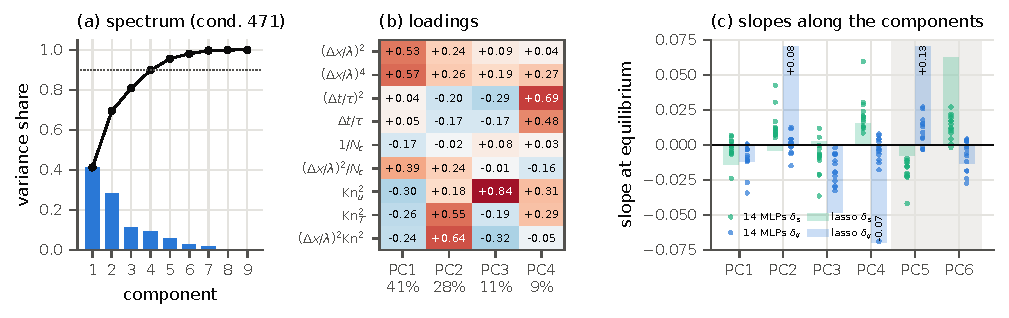
\includegraphics[width=\textwidth]{figures/fig_pca.pdf}
\caption{PCA of the training inputs: (a) variance; (b) first four components; (c) each model's
sensitivity along each component (dots: 14 sweep networks; bars: seven-term lasso).}
\label{fig:pca}
\end{figure}

When inputs move together a lasso can give their shared effect to any one of them, and small
changes in the data change which (the Gauss--Newton sign flips). Along the third
to fifth components the lasso's heat-flux coefficients are about ten times the networks'
sensitivities, while the 14 networks agree in sign on the main directions
(Figure~\ref{fig:pca}c). The correlations do not make a linear model meaningless, but
they prevent reliable attribution to individual mechanisms, so we read the models along the
principal components instead. We did not retrain on components: on all of them a linear model is unchanged, and dropping
some cannot fix the out-of-range failure below.

A Gaussian mixture model~\citep{pedregosa2011} describes the data as overlapping Gaussian
clusters. We fitted six to the training cells for
readability (the Bayesian information criterion~\citep{schwarz1978} improves up to ten: a
continuum, not separate groups). The clusters are physical regimes (Figure~\ref{fig:gate}b): shear-wave cells dominated by time step and particle
count (G2), large cells in shocks at $4\lambda_1$ (G3, G4), shock cores where gradients and cell
size combine (G6), and a regime with large velocity gradients (G5). G5 makes up 84--93\% of the
unseen shocks K3, K5 and K7, all at $\dx=\lambda_1$, but in training it appears only in the weak
shock K1 and the shear waves. \emph{The training set contains no strong shock at
$\dx=\lambda_1$.}

\begin{figure}[!t]
\centering
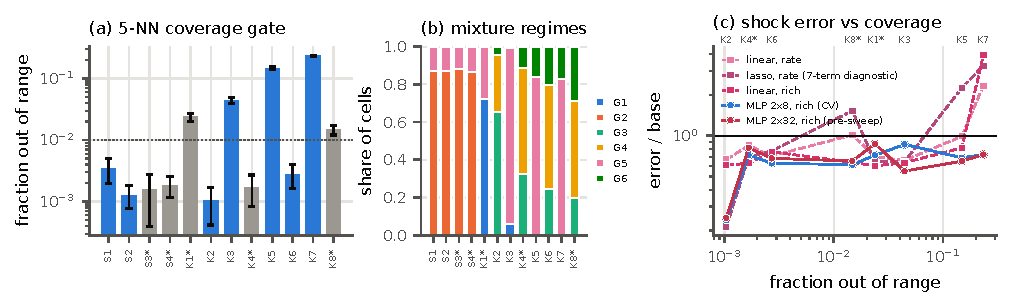
\includegraphics[width=\textwidth]{figures/fig_gate.pdf}
\caption{(a) Share of each flow's cells flagged by the coverage gate (90\% interval; grey:
training flows). (b) Cells in six Gaussian-mixture regimes. (c) Shock error against (a).}
\label{fig:gate}
\end{figure}


The mixture's likelihood flagged 56--99\% of every unseen shock, because each training flow is
a thin island in input space. A simpler test works: a cell is
out of range if its 5th-nearest training cell is farther away than for 99\% of training cells
that were left out of the fit. This \emph{coverage gate} flags K7 (23.3\% of cells, 90\% interval
22.6--24.0\%) and K5 (14.8\%, 14.1--15.6\%), cells whose temperature-gradient inputs exceed the
training range, and no other flow above 4.4\% (Figure~\ref{fig:gate}a). On exactly these two flows every linear model is worse than no correction
(1.5--2.7), while the networks still improve on it (0.69--0.71). Both models are bounded by $B$ (a factor $e^2$ on the rates), but the
linear correction grows in proportion to its inputs until far outside the training range, while
the network's hidden $\tanh$ units saturate near the edge of the training data, keeping its output
near trained values. Elsewhere the two perform similarly. The gate needs only a base-operator run.

% =========================================================================================
\section{Failure analysis: the worst slice}

We sliced the unseen shocks by the two design variables, which no model predicts: Mach number
and cell size (Table~\ref{tab:slices}). With two or three flows per slice, intervals describe these flows, not shocks in general.

\begin{table}[H]
\centering\small
\caption{Unseen shocks by Mach number and cell size: error relative to the base [90\%
interval]; red: each model's worst slice.}
\label{tab:slices}
\resizebox{\textwidth}{!}{\begin{tabular}{@{}llcccccc@{}}
\toprule
slice & flows & runs & linear, rate & lasso, rate (7-term diagnostic) & linear, rich & MLP 2x8, rich (CV) & MLP 2x32, rich (pre-sweep) \\
\midrule
Mach 1.5--3 & K2, K3 & 64 & 0.66 [0.45, 0.98] & 0.37 [0.12, 1.12] & 0.62 [0.38, 1.01] & 0.45 [0.13, 1.63] & 0.37 [0.16, 0.84] \\
Mach 6--10 & K5, K6, K7 & 96 & 1.18 [1.14, 1.22] & 1.79 [1.73, 1.85] & 1.34 [1.29, 1.40] & 0.68 [0.65, 0.71] & 0.68 [0.65, 0.72] \\
$\Delta x=4\lambda_1$ & K2, K6 & 64 & 0.69 [0.47, 1.01] & 0.41 [0.13, 1.23] & 0.68 [0.42, 1.10] & 0.39 [0.11, 1.39] & 0.41 [0.18, 0.94] \\
$\Delta x=\lambda_1$ & K3, K5, K7 & 96 & 1.15 [1.09, 1.21] & 1.68 [1.59, 1.78] & 1.26 [1.20, 1.33] & \worst{0.76 [0.72, 0.79]} & 0.64 [0.59, 0.68] \\
Mach 6--10 and $\Delta x=\lambda_1$ & K5, K7 & 64 & \worst{1.52 [1.47, 1.58]} & \worst{2.72 [2.64, 2.80]} & \worst{1.79 [1.72, 1.86]} & 0.71 [0.68, 0.73] & \worst{0.69 [0.65, 0.72]} \\
\bottomrule
\end{tabular}
}
\end{table}

The worst slice of the linear models and the $2\times32$ is Mach 6--10 at $\dx=\lambda_1$ (K5, K7; 64 runs; linear models 1.5--2.7 times worse than no correction); for the cross-validated
network it is all shocks at $\dx=\lambda_1$ (0.76). Two causes combine: a shift of the input distribution (the regime is covered in training only
by a weak shock, and the temperature-gradient inputs reach 2--7 times their training maximum),
and a model limitation (the most non-equilibrium cells, where correcting a relaxation toward a
Gaussian helps least).


% =========================================================================================
\section{The decision: a recommendation and what would reverse it}\label{sec:decision}

We recommend a procedure, in this order. (1)~Run the base operator on the new flow and compute
its coverage score. (2)~Where shocks are resolved by the cells
($\dx\approx\lambda_1$), use plain NTC, the most accurate scheme there; for strong shocks in
coarse cells, use NTC with adjacent pairing. (3)~Elsewhere, if the coverage score is low (below
about 10\%, a provisional threshold set after seeing the data), use the cross-validated network;
in shear-dominated flows (micro-devices) a linear model is an acceptable, readable alternative.
(4)~If the score is high, use a classical scheme validated for that regime, or fine DSMC where
none is. (5)~Check key points against fine runs with an absolute tolerance in the direction that
matters. We prefer the network for robustness: the linear models tie in range but fail silently outside it.

On the cylinder (Table~\ref{tab:circle}; so far only the pre-sweep $2\times32$), Fokker--Planck
operators predict the $2\lambda$ heat load within 3\% (NTC $+15\%$), but the $2\times32$'s $-3\%$
is on the unsafe side: the recommended network must be run there before use for heating. One fact would reverse this: a population shift. If an application puts many cells out of range
(e.g.\ dense gas at a cooled wall, cells $\sim30\lambda$), no learned model is validated there.

\bibliographystyle{unsrtnat}
\bibliography{refs}

% =========================================================================================
\clearpage
\appendix

\section{DSMC and the collision operators}\label{app:dsmc}

The velocity distribution $f(x,v,t)$ obeys the Boltzmann equation
$\partial_tf+v\cdot\nabla_xf=Q(f,f)$, with $Q$ the binary collision integral. DSMC splits each
step $\Delta t$ into free flight, $x_i\leftarrow x_i+v_i\Delta t$ with wall and inflow
boundaries, and collisions within cells~\citep{bird1994}. In the no-time-counter (NTC) scheme a
cell with $N_c$ particles, each standing for $F_N$ molecules, tests
$\tfrac12N_c(N_c-1)F_N(\sigma_Tg)_\mathrm{max}\Delta t/V_c$ candidate pairs. Each is accepted
with probability $\sigma_Tg/(\sigma_Tg)_\mathrm{max}$, where $g$ is the relative speed and
$\sigma_T$ the cross-section, and is scattered with the variable-soft-sphere law~\citep{koura1991},
conserving momentum and energy pairwise. Pairs are drawn uniformly within the cell, which causes
the $(\dx/\lambda)^2$ transport error~\citep{alexander1998}. Adjacent pairing sorts the particles
by position and pairs neighbours.

In BGK~\citep{bgk1954} and ES-BGK~\citep{holway1966} each particle is, with probability
$1-e^{-\Delta t/\tau}$, given a new velocity drawn from a Gaussian $\mathcal N(u,\Lambda)$ with
$\Lambda=\theta I$ (BGK; Prandtl number 1) or $\Lambda=(1-\nu)\theta I+\nu\Pi/\rho$ (ES-BGK;
Prandtl number 2/3), with $\theta$ the temperature in velocity units and $\Pi$ the stress
tensor; a projection then restores conservation. ``+recon'' replaces the cell velocity $u_c$ by
the linear interpolation $u(x_i)=u_c+G_c(x_i-\bar x_c)$ from neighbouring cells.

The ES Fokker--Planck operator~\citep{jenny2010,gorji2011,mathiaud2016}, our base, moves every
particle's velocity relative to the local mean, $c_i=v_i-u(x_i)$, by an Ornstein--Uhlenbeck
process integrated exactly over a step:
\begin{equation}
c_i'=a\,c_i+\mathrm{chol}(\Sigma)\,\xi_i,\qquad \Sigma=\theta(1-a^2)I+(e_s-a^2)\Pi_\mathrm{dev},
\qquad a=e^{-r_q\Delta t/3},\ e_s=e^{-r_s\Delta t},
\end{equation}
with $\xi_i\sim\mathcal N(0,I)$, $r_s=p/\mu(T)$, $r_q=\mathrm{Pr}\,p/\mu(T)$, $\mathrm{Pr}=2/3$,
a limiter that keeps $\Sigma$ positive definite~\citep{mathiaud2016}, and a final projection that
restores each cell's momentum and energy exactly. The stress then relaxes at rate $r_s$ and the
heat flux at $r_q$ for any $\Delta t$. The learned outputs multiply $r_s$ and $r_q$ by
$e^{\delta_s}$ and $e^{\delta_q}$, and, before the projection, impose a stress target
$\Pi^*/\theta=\sum_k\alpha_kT_k$ on four Burnett tensor bases (by a symmetric stretch
$c\to(I+K)c$), impose a heat-flux target on three vector bases (by a Hermite drift), scale the
velocity interpolation, add a temperature interpolation to the noise, and reshape the noise's
radial distribution (kurtosis 11--38 against the Gaussian's 15). All are zero at initialisation.

\section{Training through the solver}\label{app:ad}

The solver is written in JAX. A training window of $W=100$ steps is a checkpointed loop whose
random numbers are regenerated during the backward pass, so reverse-mode AD~\citep{griewank2008}
gives the exact derivative of the window's fluxes with respect to $\theta$ through collisions,
free flight and inflow. Discrete events (which cell a particle is in, wall hits) carry no
gradient. AD agrees with finite differences using common random numbers to seven digits. Two
independent copies of each window give an unbiased estimate of $\mathbb E[d]^2$,
$\mathbb E[d_ad_b]$, used for monitoring. The gradient uses
$b\,\partial m/\partial\theta$, where $b$ is a running mean of $d$ for each flow, window time and
wave mode or cell, held fixed in the derivative; its standard error was 10--20 times lower than
that of the two-copy product. Shock windows continue persistent coarse simulations, so the model
is trained on its own steady state: windows started from fine snapshots never reached the
steady heat-flux deficit (total $q_x$ 1.01 of the reference in the window, 0.94 at steady state).
Each iteration uses 32 windows per flow. The optimiser is Adam with each layer's step divided by
its number of inputs, and the final parameters are the mean of the last 25\% of iterates.

\section{Additional results}\label{app:extra}

\begin{table}[H]
\centering\small
\caption{The nine network settings: error relative to the base on the training flows (networks
trained on all five) and on the left-out flow (mean over LOCO folds $\pm$ standard error),
measured with the shorter validation runs (uncorrected operator: 1.17).}
\label{tab:sweep}
\begin{tabular}{@{}lrcc@{}}
\toprule
design point (depth$\times$width, weight decay, learning rate) & parameters & training & held-out \\
\midrule
1$\times$8, 0, 0.001 & 204 & 0.69 & 0.81$\pm$0.13 \\
1$\times$32, 0.001, 0.003 & 780 & 0.57 & 0.57$\pm$0.45 \\
1$\times$128, 0.01, 0.01 & 3084 & 0.60 & 0.76$\pm$0.28 \\
2$\times$8, 0.001, 0.01 & 276 & 0.64 & 0.57$\pm$0.23 \\
2$\times$32, 0.01, 0.001 & 1836 & 1.17 & 1.03$\pm$0.07 \\
2$\times$128, 0, 0.003 & 19596 & 0.57 & 0.73$\pm$0.22 \\
3$\times$8, 0.01, 0.003 & 348 & 1.17 & 1.22$\pm$0.09 \\
3$\times$32, 0, 0.01 & 2892 & 0.43 & 0.95$\pm$0.15 \\
3$\times$128, 0.001, 0.001 & 36108 & 0.74 & 0.69$\pm$0.33 \\
\bottomrule
\end{tabular}

\end{table}

\begin{table}[H]
\centering\small
\caption{Mach 10 argon cylinder at Knudsen number 0.04, wall at half the stagnation temperature:
drag and heat load relative to a fine NTC simulation ($\pm$ standard error) with every cell
$2\lambda$ or $4\lambda$ wide. The learned operator runs in every cell, including the cold layer
next to the wall, which is outside its training range. With $2\lambda$ cells, every
Fokker--Planck-based operator predicts the heat load far better than NTC (+15\%); the learned
corrections are within about two standard errors of their base.}
\label{tab:circle}
\begin{tabular}{@{}lcccc@{}}
\toprule
operator & drag, $2\lambda$ & drag, $4\lambda$ & heat, $2\lambda$ & heat, $4\lambda$ \\
\midrule
NTC & 1.034$\pm$0.007 & 1.041$\pm$0.016 & 1.146$\pm$0.023 & 1.245$\pm$0.047 \\
ES-BGK + recon & 1.011$\pm$0.008 & 1.054$\pm$0.017 & 1.061$\pm$0.023 & 1.184$\pm$0.049 \\
ES-FP + recon (base) & 1.007$\pm$0.008 & 1.046$\pm$0.018 & 1.027$\pm$0.022 & 1.151$\pm$0.048 \\
linear, rate & 1.005$\pm$0.007 & 1.021$\pm$0.016 & 0.998$\pm$0.021 & 1.141$\pm$0.048 \\
MLP 2x32, rich (pre-sweep) & 1.004$\pm$0.008 & 1.011$\pm$0.015 & 0.969$\pm$0.020 & 1.129$\pm$0.046 \\
\bottomrule
\end{tabular}

\end{table}

\begin{figure}[H]
\centering
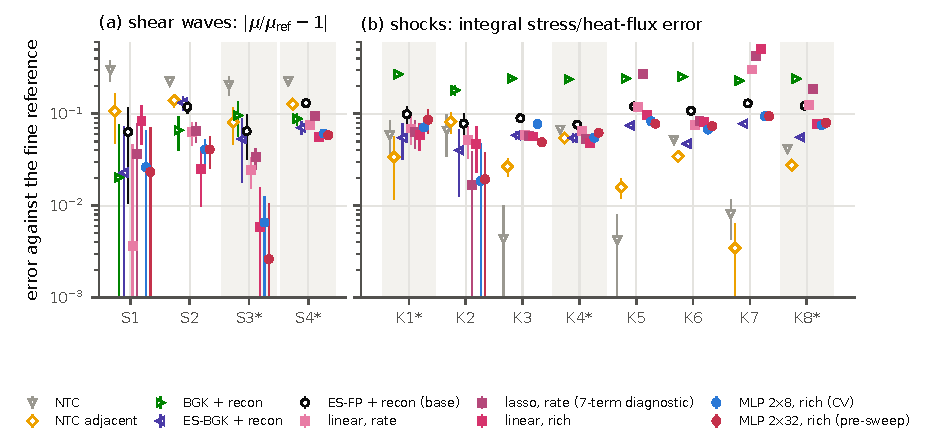
\includegraphics[width=\textwidth]{figures/fig_performance.pdf}
\caption{Absolute error of every operator on the twelve flows (512 runs per shear wave, 64 for
the classical schemes on S3 and S4; 32 long runs per shock; $\pm1$ standard error;
* and grey background: training flows). Hollow: classical schemes; squares: linear models;
filled circles: networks.}
\label{fig:perf}
\end{figure}

\section{Reproducibility and acknowledgements}\label{app:repro}

This work used the Alpine high-performance computing resource at the University of Colorado
Boulder (CURC).

{\sloppy\textbf{Code and data.} The code is the branch \texttt{neural-collision} of
\url{https://github.com/missle2/JAX-DSMC/tree/neural-collision}. The operators and inputs are in
\texttt{jax\_dsmc/collide/relax.py}; the flows, training, lasso, evaluation and cylinder drivers
in \texttt{examples/learned\_collision/}; every cluster job's exact command in
\texttt{examples/mesh/cluster/study.py}; the unsupervised analysis in
\texttt{scratch/lc\_cellfeat.py} and \texttt{scratch/lc\_unsup.py}; the figures and tables in
\texttt{docs/learning\_report/make\_figures.py}. Run outputs are not in git: the result files
behind every figure and table (all JSON results and the per-cell inputs, 33~MB) are the release
asset \texttt{lc\_results\_2026-11-15.tar.gz} (SHA-256 \texttt{9b22f269\ldots a9dd0}). The fine
reference snapshots (6~GB) are not distributed; step~3 regenerates them.\par}

\textbf{Seeds.} Every driver uses fixed seeds: training, the warm pool, the input statistics and
the lasso use \texttt{--seed 0} by default; the all-flow sweep runs use seeds 0 and 1; shear-wave evaluations use run indices $0,\dots,N-1$ and shock evaluations draw their starts from NumPy seed 0; the analysis uses NumPy seed 0. Results are reproducible to
floating-point differences between GPU models.

\textbf{1. Figures and tables from the released results} (any machine, CPU, about ten minutes).
The headline result (Table~\ref{tab:headline}) is printed to the terminal and written to
\texttt{docs/learning\_report/tables/headline.tex}.
{\footnotesize
\begin{verbatim}
git clone -b neural-collision https://github.com/missle2/JAX-DSMC.git
cd JAX-DSMC
python3 -m venv .venv && source .venv/bin/activate          # Python >= 3.10
pip install --upgrade pip
pip install "jax==0.6.2" flax==0.10.7 optax==0.2.8 numpy==2.2.6 scipy==1.15.3 \
            matplotlib==3.10.9 scikit-learn==1.7.2
curl -LO https://github.com/missle2/JAX-DSMC/releases/download/learned-collision-report/\
lc_results_2026-11-15.tar.gz
sha256sum lc_results_2026-11-15.tar.gz      # 9b22f2699f951782bb72b352ff0eab83...
tar -xzf lc_results_2026-11-15.tar.gz       # -> examples/learned_collision/results/
JAX_ENABLE_X64=1 JAX_PLATFORMS=cpu PYTHONPATH=. python3 docs/learning_report/make_figures.py
(cd docs/learning_report && latexmk -pdf report.tex)
\end{verbatim}}

\textbf{2. Environment on a GPU cluster.} The simulations need NVIDIA GPUs with a CUDA~12
driver; every job fits one GPU (24~GB), except the fine cylinders (48~GB). On a login node:
{\footnotesize
\begin{verbatim}
git clone -b neural-collision https://github.com/missle2/JAX-DSMC.git && cd JAX-DSMC
module load python                     # site-specific: any Python >= 3.10
python3 -m venv $HOME/jax-env && source $HOME/jax-env/bin/activate
pip install --upgrade pip
pip install "jax[cuda12]==0.6.2" flax==0.10.7 optax==0.2.8 numpy==2.2.6 scipy==1.15.3 \
            matplotlib==3.10.9 scikit-learn==1.7.2
# the sweep's plan (which runs, how many iterations) from the release archive:
curl -LO https://github.com/missle2/JAX-DSMC/releases/download/learned-collision-report/\
lc_results_2026-11-15.tar.gz
tar -xzf lc_results_2026-11-15.tar.gz examples/learned_collision/results/sweep_plan_v3.json
# check that a compute node sees its GPU (expect [CudaDevice(id=0)] in check_*.out):
sbatch --job-name=check --export=ALL,CMD="python3 -c 'import jax; print(jax.devices())'" \
       docs/learning_report/run_lc.sbatch
\end{verbatim}}
Every job runs through this SLURM script (edit the account and partition lines for your site):
{\footnotesize\VerbatimInput{run_lc.sbatch}}

\textbf{3. All simulations.} \texttt{reproduce.sh} submits each stage's jobs, taking every
command from \texttt{study.py}; run the stages in order, each after the previous has finished
(\texttt{squeue -u \$USER}), and \texttt{DRY=1} prints the jobs without submitting. The sweep
is about 55 GPU-hours (7 jobs of 7.8~h); each Gauss--Newton lasso step about 0.5~h.
{\footnotesize\VerbatimInput{reproduce.sh}}

\textbf{The headline model alone.} After stages \texttt{refs} and \texttt{prep}, the
cross-validated network of Table~\ref{tab:headline} is trained and evaluated by
{\footnotesize
\begin{verbatim}
LC="python3 -m examples.learned_collision"
for s in 0 1; do
  $LC.train --model mlp --depth 2 --width 8 --weight-decay 0.001 --lr 0.01 --iters 177 \
    --cases S3 S4 K1 K4 K8 --validate-train --seed $s --tag cv_v3_p3_all_s$s \
    --outputs rich --features features_v4.json --warm-pool v1
  $LC.evaluate --cases S1 S2 S3 S4 K1 K2 K3 K4 K5 K6 K7 K8 --operators \
    --theta train_mlp_cv_v3_p3_all_s$s.json --seeds 512 --tag test_v3p3_s$s
done
\end{verbatim}}
(each line as the \texttt{CMD} of a \texttt{run\_lc.sbatch} job), followed by stage
\texttt{analysis}.

\section{Use of generative AI}

An AI coding assistant (Claude, primarily using Opus 5.5 via Claude Code) was used throughout: to implement solver features (the BGK and
ES-BGK operators, the inputs, the twelve-output correction), the training, lasso and evaluation
drivers and the cluster job definitions; to analyse results and make figures; for literature review; and to draft this
report. Architecture of the models, the choice of training approach, and other higher level decisions were not made by Claude. Some of the errors it made, and how they were caught:
\begin{itemize}
\item \emph{A wrong gradient}: a stop-gradient on the positive-definiteness limiter made AD
differ from finite differences by $\sim10^3$ wherever the limiter was active; caught by the
AD-versus-finite-difference test required before any training.
\item \emph{Anti-correlated copies}: the persistent-shock code compared two independent
simulations against one target placed at their mean shock position, creating a fake bias;
caught because the two-copy loss, which must be non-negative, drifted negative in every such
run. All affected runs were discarded and rerun.
\item \emph{Interpretability of the Lasso}: The agent initially suggested an interpretation of the lasso coefficients as a ranking of 
predictive power, which is not correct given the correlations; caught by checking the course's notes on lasso interpretation.
\item \emph{A wrong PCA}: its first account of the principal components came from an uncentred
correlation matrix; caught when the analysis was redone on the per-cell data.
\item \emph{An over-strict novelty test}: the Gaussian-mixture likelihood flagged most unseen
cells; caught by comparing it with simpler range and nearest-neighbour tests.
\item \emph{An untuned headline model}: a network not chosen by cross-validation was first
reported as the best model; caught while checking the report against the course's requirement of honestly tuned models, after which
the cross-validated choice was evaluated on all flows.
\end{itemize}

\end{document}
